\chapter{Horizontes, ecuación de estado y energía del vacío}

\section{Marco preferente, recesión superlumínica y horizonte}

La radiación cósmica de fondo de microondas sí determina un marco especial. En el marco en que esa radiación se observa isotrópica, las galaxias cercanas también están, en promedio, en reposo. Si nos movemos a través del fondo, los fotones que llegan de frente experimentan un desplazamiento Doppler hacia energías mayores, y los que llegan desde atrás, hacia energías menores. El marco preferente es aquel en que el fondo de microondas se observa isotrópico y, además, es también, en promedio, el marco en que las galaxias locales están en reposo.

\begin{classroomqa}
\lecturetimestamp{00:00:25}
\audiencequestion{¿La longitud de onda aparente de la radiación cósmica depende del movimiento del observador? ¿Implica eso que existe un marco preferente?}
\lecturerresponse{Sí. El movimiento a través del fondo de microondas produce una anisotropía Doppler, así que existe un marco cosmológico preferente: aquel en que el fondo de microondas se observa isotrópico. Además, es también, en promedio, el marco en que las galaxias locales están en reposo.}
\end{classroomqa}

Una segunda cuestión se refiere a las velocidades de recesión. La ley de Hubble dice que galaxias suficientemente distantes se separan de acuerdo con
\begin{equation}
v = H d .
\end{equation}
Para valores suficientemente grandes de \(d\), esta velocidad de recesión supera la velocidad de la luz. Esto no contradice la relatividad, porque la prohibición es local: un objeto no puede pasar junto a otro, justo delante de nosotros, a una velocidad superior a la de la luz. La afirmación sobre galaxias distantes se refiere a la geometría entre lugares muy separados.

\begin{classroomqa}
\lecturetimestamp{00:04:48}
\audiencequestion{¿Pueden dos galaxias tener una velocidad relativa mayor que \(c\)?}
\lecturerresponse{Sí, si están lo bastante alejadas. La recesión de Hubble puede superar la velocidad de la luz sin violar la relatividad local; el lugar donde la velocidad de recesión alcanza \(c\) es un horizonte.}
\end{classroomqa}

Cuando la recesión alcanza la velocidad de la luz, las señales enviadas hacia nosotros dejan de acercarse en términos netos. El rayo sigue moviéndose localmente a la velocidad límite, pero la distancia que debe recorrer crece demasiado deprisa.

\begin{classroomqa}
\lecturetimestamp{00:07:03}
\audiencequestion{¿No seguiría viajando hacia nosotros un rayo de luz enviado en sentido contrario?}
\lecturerresponse{Localmente sí, pero el espacio se expande más deprisa de lo que el rayo puede avanzar. El rayo se mueve a la velocidad límite respecto a los puntos cercanos, mientras que la distancia total hasta nosotros sigue aumentando.}
\end{classroomqa}

\section{La métrica en expansión y la analogía de la línea}

Una imagen útil es la de una dimensión. Imaginemos una línea formada por átomos. Si estiramos una línea de material corriente, al final se rompe. Modifiquemos ahora la imagen: cada vez que los átomos vecinos se separan demasiado, insertamos otro entre ellos. La línea sigue creciendo, pero sus propiedades locales no se diluyen.

\begin{figure}
\centering
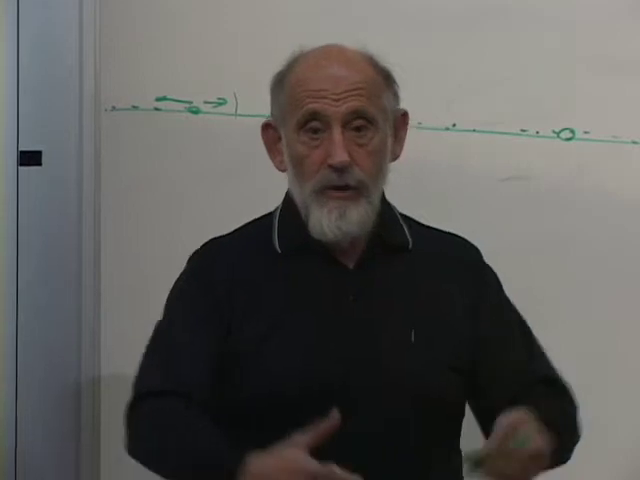
\includegraphics[width=0.60\textwidth]{lecture_04_figure_02.png}
\caption{Línea unidimensional utilizada para representar una métrica en expansión.}
\end{figure}

En esta imagen sigue habiendo una velocidad límite local para las señales, igual que el sonido tiene una velocidad límite en una línea corriente. La regla es local: una perturbación no puede superar esa velocidad respecto a los puntos cercanos. Sin embargo, si la línea es lo bastante larga y se insertan puntos nuevos con suficiente rapidez, las partes suficientemente distantes se alejan tan deprisa que una señal nunca puede regresar.

Por tanto, la suma de velocidades de la relatividad especial es solo una parte de la historia. Se aplica localmente, cuando los observadores pasan uno junto al otro en el mismo punto. No es la herramienta adecuada para describir galaxias muy separadas en una geometría en expansión.

\begin{classroomqa}
\lecturetimestamp{00:09:42}
\audiencequestion{¿Sigue siendo válida en esta situación la ley relativista habitual de suma de velocidades?}
\lecturerresponse{Localmente, en un punto, sí. Si los observadores pasan uno junto al otro, uno tras otro, se aplica la regla habitual de la relatividad especial. Pero no es la manera adecuada de describir una recesión superlumínica entre objetos muy separados; en ese caso hay que volver a la geometría del espacio en expansión.\(c\)
}
\end{classroomqa}

La misma imagen ofrece una explicación sencilla del corrimiento al rojo. Dibujemos una onda sobre la línea. Al expandirse la línea, también aumenta la longitud de onda. En una geometría en expansión, no se trata solo de una imagen sugerente: las ecuaciones de onda en un espacio-tiempo en expansión producen realmente longitudes de onda estiradas.

\begin{classroomqa}
\lecturetimestamp{00:14:42}
\audiencequestion{¿La afirmación de que una onda se estira junto con el universo es teórica, empírica o ambas cosas?}
\lecturerresponse{Es una consecuencia teórica de la propagación de ondas en un espacio-tiempo en expansión y, además, cuenta con el respaldo de las observaciones astronómicas.}
\end{classroomqa}

Esta imagen no representa una banda elástica. Al estirarla, una banda elástica se hace más delgada, y alguien que viviera en ese medio vería cambiar sus propiedades locales. Aquí las propiedades locales permanecen iguales mientras crece la escala global de distancias.

\section{La última dispersión y el universo observable}

El horizonte es el lugar donde la recesión alcanza la velocidad de la luz. La superficie de última dispersión se encuentra ligeramente dentro de él. Una señal emitida desde el horizonte sufriría un corrimiento al rojo ilimitado; la radiación de última dispersión tiene un corrimiento al rojo enorme, pero finito.

\begin{classroomqa}
\lecturetimestamp{00:17:53}
\audiencequestion{¿Qué relación hay entre la recesión superlumínica, la superficie de última dispersión y el universo observable?}
\lecturerresponse{El horizonte es el lugar donde la recesión alcanza la velocidad de la luz. La superficie de última dispersión se encuentra ligeramente dentro de él porque su corrimiento al rojo es enorme, pero finito. A efectos prácticos, marca el borde del universo observable.}
\end{classroomqa}

El corrimiento al rojo de la radiación de última dispersión es, aproximadamente, un factor \(10^3\). Es un valor tan grande que, para muchos propósitos, la superficie de última dispersión está muy cerca del horizonte. El universo observable es la parte del universo desde la que la luz puede llegar hasta nosotros.

En tiempos tardíos, la expansión se aproxima al régimen dominado por el vacío. Entonces la magnitud de Hubble tiende a una constante, el horizonte se aproxima a un tamaño fijo y tanto las galaxias como la radiación de microondas van desapareciendo progresivamente de nuestra vista.

\begin{classroomqa}
\lecturetimestamp{00:22:43}
\audiencequestion{Puesto que \(H\) cambia con el tiempo, ¿cambia también la distancia al horizonte? ¿Acabará desapareciendo el fondo de microondas?}
\lecturerresponse{En tiempos tardíos, \(H\) tiende a una constante, así que el horizonte se aproxima a una distancia fija. El fondo de microondas sigue estirándose, enfriándose y desvaneciéndose. Las galaxias distantes también atraviesan el horizonte y desaparecen de nuestra vista.}
\end{classroomqa}

Solo permanecen visibles las estructuras que ya están ligadas gravitatoriamente. El sistema solar no se desintegra, ni tampoco la galaxia, pero el universo a gran escala se convierte en una isla aislada.

\section{La ecuación básica de expansión y los tres componentes}

La ecuación básica de expansión es ahora
\begin{equation}
\left(\frac{\dot a}{a}\right)^2 = \frac{8\pi G}{3}\rho ,
\qquad c=1 .
\end{equation}
Aquí \(a(t)\) es el factor de escala y \(\rho\) es la densidad de energía total.

\begin{figure}
\centering
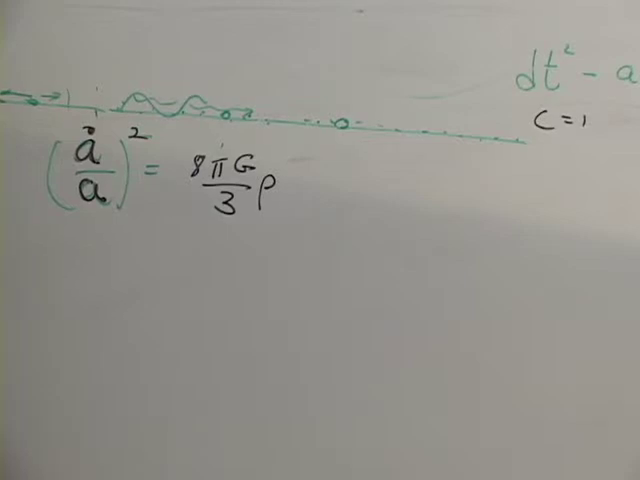
\includegraphics[width=0.74\textwidth]{lecture_04_figure_03.png}
\caption{Ecuación básica de expansión junto con la analogía de la línea unidimensional.}
\end{figure}

Hay tres componentes dinámicamente importantes.

Para la materia,
\begin{equation}
\rho=\frac{\text{const.}}{a^3},
\qquad
a(t)\sim t^{2/3}.
\end{equation}
Este es el caso de objetos masivos que se mueven con la expansión global y que están esencialmente en reposo en el marco comóvil.

Para la radiación,
\begin{equation}
\rho=\frac{\text{const.}}{a^4},
\qquad
a(t)\sim t^{1/2}.
\end{equation}
La potencia adicional de \(a\) se debe al corrimiento al rojo que experimenta cada fotón al expandirse el universo.

También hay
\begin{equation}
\rho_0=\text{constant},
\end{equation}
energía del vacío, también llamada energía oscura o, salvo factores numéricos convencionales, constante cosmológica. Este componente no se diluye en absoluto.

El siguiente paso es relacionar la densidad de energía con la presión.

\section{La presión de radiación y la materia fría}

Empecemos por la radiación. Consideremos una caja unidimensional, solo un segmento de longitud \(L\), que contiene fotones rebotando de un lado a otro. En una dimensión, fuerza y presión son, en la práctica, lo mismo.

Tomemos un fotón cuyo módulo del momento es \(p\). Cuando se refleja en una pared, su momento cambia en
\begin{equation}
\Delta p = 2p.
\end{equation}
El tiempo entre colisiones sucesivas con la misma pared es
\begin{equation}
\Delta t = \frac{2L}{c}.
\end{equation}
Por tanto, la fuerza media sobre la pared es
\begin{equation}
F=\frac{\Delta p}{\Delta t}=\frac{pc}{L}.
\end{equation}
Para un fotón,
\begin{equation}
E=pc,
\end{equation}
así que
\begin{equation}
F=\frac{E}{L}.
\end{equation}
La energía dividida por la longitud es la densidad de energía unidimensional. En este caso unidimensional,
\begin{equation}
P=\rho .
\end{equation}

Con muchos fotones, la misma relación se mantiene al promediar. La fuerza total es simplemente la energía total por unidad de longitud.

Pasemos ahora a tres dimensiones. Si todos los fotones se movieran solo a lo largo de un eje, ejercerían presión sobre un par de caras y ninguna sobre las demás. Este supuesto es deliberadamente incorrecto, pero muestra enseguida qué hay que corregir. En un baño isotrópico, el momento se distribuye en todas las direcciones. En promedio, un tercio de la densidad de energía contribuye a cada componente de la presión. El resultado es
\begin{equation}
P=\frac{\rho}{3}.
\end{equation}

Para la materia fría, el resultado es distinto. Tomemos una caja comóvil, una pequeña región que se mueve con el flujo del universo. Las partículas de su interior tienen energía, pero, si están en reposo respecto a la caja, no chocan contra sus paredes. Por tanto, la presión es
\begin{equation}
P=0.
\end{equation}

\begin{figure}
\centering
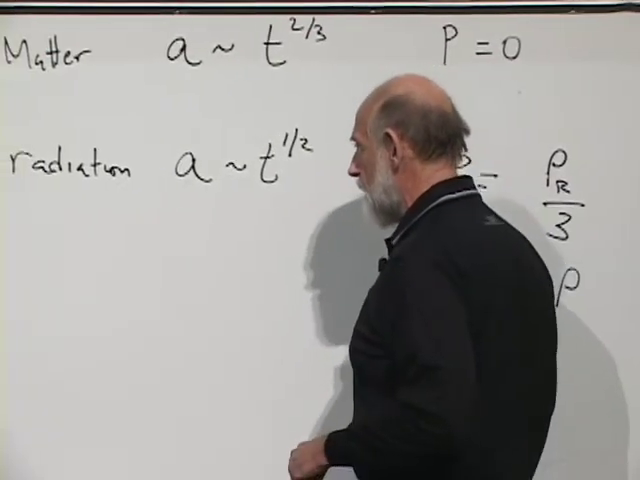
\includegraphics[width=0.74\textwidth]{lecture_04_figure_04.png}
\caption{Materia y radiación: \(a\sim t^{2/3}\), \(P=0\) y \(a\sim t^{1/2}\), \(P=\rho/3\).}
\end{figure}

El resumen de la pizarra es
\begin{align}
\text{matter:}\qquad & a(t)\sim t^{2/3}, \qquad P=0,\\
\text{radiation:}\qquad & a(t)\sim t^{1/2}, \qquad P=\frac{\rho}{3}.
\end{align}

\begin{classroomqa}
\lecturetimestamp{00:54:27}
\audiencequestion{En el universo en expansión, ¿no se están separando realmente las partículas?}
\lecturerresponse{Sí, pero el argumento sobre la presión se aplica a una caja comóvil infinitesimal. A esa escala local, el razonamiento termodinámico sigue siendo válido.}
\end{classroomqa}

\section{La ecuación de estado}

Se supone que la presión es proporcional a la densidad de energía:
\begin{equation}
P=w\rho .
\end{equation}
En la pizarra, el mismo parámetro se escribe como \(\omega\). Para los dos casos básicos,
\begin{equation}
w=0 \quad \text{for cold matter},
\qquad
w=\frac{1}{3} \quad \text{for radiation}.
\end{equation}

También son posibles los casos intermedios. Los valores comprendidos entre \(0\) y \(1/3\) describen materia que no es ni completamente fría ni plenamente relativista. Aquí se menciona como ejemplo la materia oscura caliente.

\begin{figure}
\centering
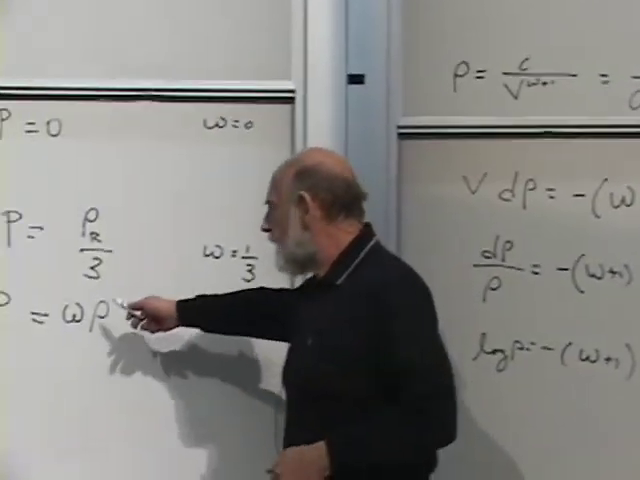
\includegraphics[width=0.74\textwidth]{lecture_04_figure_05.png}
\caption{Ecuación de estado \(P=\omega\rho\) junto con el argumento sobre la escala de la densidad.}
\end{figure}

La siguiente cuestión es si \(w\) determina la dependencia de \(\rho\) respecto de \(a\). La respuesta se obtiene de una identidad termodinámica.

Tomemos una caja de volumen \(V\). Si su contenido ejerce una presión \(P\), cuando la caja se expande en \(dV\), el trabajo realizado sobre sus paredes es
\begin{equation}
dE=-P\,dV.
\end{equation}
Escribamos ahora la energía como
\begin{equation}
E=\rho V.
\end{equation}
Su diferencial es
\begin{equation}
dE=\rho\,dV+V\,d\rho .
\end{equation}
Al igualar las dos expresiones se obtiene
\begin{equation}
\rho\,dV+V\,d\rho=-P\,dV,
\end{equation}
o bien
\begin{equation}
V\,d\rho=-(\rho+P)\,dV.
\end{equation}
Usando \(P=w\rho\),
\begin{equation}
V\,d\rho=-(1+w)\rho\,dV.
\end{equation}
Dividamos por \(\rho V\):
\begin{equation}
\frac{d\rho}{\rho}=-(1+w)\frac{dV}{V}.
\end{equation}
Al integrar,
\begin{equation}
\rho \propto V^{-(1+w)}.
\end{equation}
Para una caja cosmológica comóvil,
\begin{equation}
V\propto a^3,
\end{equation}
y, por tanto,
\begin{equation}
\rho \propto a^{-3(1+w)}.
\end{equation}

Se recuperan enseguida los casos anteriores:
\begin{align}
w=0 &\Longrightarrow \rho \propto a^{-3},\\
w=\frac{1}{3} &\Longrightarrow \rho \propto a^{-4}.
\end{align}

Por eso importa \(w\). Una vez conocida \(\rho(a)\), se puede sustituir en la ecuación de Friedmann. Después se prueba una ley de potencias \(a\sim t^\alpha\) y se determina cómo se expande el universo para esa ecuación de estado.

\section{Energía del vacío y presión negativa}

Un caso especial se comporta de manera distinta:
\begin{equation}
w=-1.
\end{equation}
Entonces
\begin{equation}
1+w=0,
\end{equation}
por lo que el exponente se anula y
\begin{equation}
\rho=\rho_0=\text{constant}.
\end{equation}
La presión correspondiente es
\begin{equation}
P=-\rho .
\end{equation}

La presión negativa no tiene nada de misterioso por sí misma. La presión positiva empuja hacia fuera las paredes de una caja. La negativa tira de ellas hacia dentro. Es tensión. Una banda elástica estirada es un ejemplo cotidiano: almacena energía positiva, pero tira de sus extremos para juntarlos.

Sustituyamos la densidad constante \(\rho_0\) en la ecuación de Friedmann:
\begin{equation}
\left(\frac{\dot a}{a}\right)^2=\frac{8\pi G}{3}\rho_0.
\end{equation}
El miembro derecho es simplemente un número, así que
\begin{equation}
\frac{\dot a}{a}=\sqrt{\frac{8\pi G}{3}\rho_0}.
\end{equation}
Este es el caso especial en que la magnitud de Hubble sí es constante. La ecuación puede escribirse como
\begin{equation}
\dot a=\sqrt{\frac{8\pi G}{3}\rho_0}\,a,
\end{equation}
y la solución es
\begin{equation}
a(t)\propto \exp\!\left(\sqrt{\frac{8\pi G}{3}\rho_0}\,t\right).
\end{equation}

Esta es una expansión exponencial. La escala de tiempo pertinente es el tiempo de crecimiento por un factor \(e\), no el tiempo de duplicación; la estimación aproximada utilizada aquí lo sitúa en el orden de la edad del universo. La energía del vacío y la constante cosmológica son el mismo ingrediente físico, salvo por convenciones numéricas históricas.

\begin{classroomqa}
\lecturetimestamp{01:27:16}
\audiencequestion{Si la energía del vacío impulsa una expansión exponencial, ¿no acabará todo desgarrado?}
\lecturerresponse{No necesariamente. Los sistemas ligados pueden resistirla. Una galaxia, un sistema solar o un átomo no tienen por qué desgarrarse, mientras que las estructuras suficientemente grandes y poco densas sí participan en la expansión y acaban separándose.}
\end{classroomqa}

\begin{classroomqa}
\lecturetimestamp{01:31:43}
\audiencequestion{¿Tiene algún significado el signo negativo al extraer la raíz cuadrada de la ecuación de Friedmann?}
\lecturerresponse{Sí. La raíz cuadrada da dos ramas. Una corresponde a la solución en expansión y la otra a la solución en contracción, que es su reversión temporal. Las propias ecuaciones admiten ambas.}
\end{classroomqa}

\section{Tres eras y la historia de expansión observada}

Los tres componentes están presentes y su densidad evoluciona de manera distinta:
\begin{equation}
\begin{aligned}
\rho_{\text{radiation}}&\propto a^{-4},\\
\rho_{\text{matter}}&\propto a^{-3},\\
\rho_0&=\text{constant}.
\end{aligned}
\end{equation}
De ahí se deducen inmediatamente tres eras.

Para valores muy pequeños de \(a\), domina la radiación. Más adelante domina la materia. Para valores suficientemente grandes de \(a\), domina la energía del vacío. Las leyes de expansión correspondientes son
\begin{equation}
a(t)\sim t^{1/2},
\qquad
a(t)\sim t^{2/3},
\qquad
a(t)\sim e^{Ht}.
\end{equation}

Los tiempos aproximados que se citan aquí son los siguientes: la radiación deja paso a la materia después de unos \(10^4\) años. El universo se vuelve transparente más tarde, después de unos \(10^5\) años. La transición del dominio de la materia a la expansión acelerada ocurre mucho más tarde, después de varios miles de millones de años, aproximadamente a mitad de la historia cósmica según la estimación de orden de magnitud que se utiliza.

¿Cómo se infiere esta historia? No podemos ver el futuro, pero sí el pasado. Mirar a mayor distancia equivale a mirar a épocas anteriores. Al observar galaxias distantes, medir cómo se relaciona su movimiento con la distancia y reconstruir la magnitud de Hubble en función del tiempo retrospectivo, se reconstruye la evolución temporal del factor de escala. La era dominada por la radiación es demasiado temprana para observarla directamente mediante la astronomía galáctica ordinaria, pero la era dominada por la materia y la transición al dominio del vacío sí se aprecian en la curva reconstruida.

\section{La última dispersión en el futuro lejano}

La evolución futura del cielo de microondas no es lo mismo que la desaparición de las galaxias al atravesar el horizonte. La radiación que vemos en épocas posteriores procede de materia más distante, así que el efecto es observar regiones más profundas y frías, en lugar de ver cómo los mismos átomos se alejan sin más.

\begin{classroomqa}
\lecturetimestamp{01:48:07}
\audiencequestion{Si la superficie de última dispersión se desvanece en el horizonte, ¿es eso lo mismo que las galaxias que se alejan más allá del horizonte?}
\lecturerresponse{No. La radiación posterior no procede de los mismos átomos que la que vemos ahora. Procede de átomos que estaban más lejos, así que es como observar regiones cada vez más profundas del universo, mientras la radiación se ve cada vez más fría.}
\end{classroomqa}

\section{Curvatura, la imagen del gran colapso y el horizonte en tiempos tardíos}

Hasta ahora se había omitido el término de curvatura. Al recuperarlo, se obtiene
\begin{equation}
\left(\frac{\dot a}{a}\right)^2
=
\frac{8\pi G}{3}\rho
-
\frac{K}{a^2}.
\end{equation}
Numéricamente, este término parece pequeño, pero conceptualmente es importante. En el lenguaje newtoniano antiguo, distingue los casos de energía total positiva, nula y negativa. En el lenguaje relativista, distingue las geometrías espaciales.

Antes de que se tomara en serio la energía del vacío, se solía imaginar un universo dominado por la materia en que la expansión acabaría invirtiéndose. De ahí surgió la antigua imagen del gran colapso: expansión desde el Big Bang y, después, recontracción. Las matemáticas siguen siendo válidas, pero ya no parece que describan nuestro universo.

\begin{classroomqa}
\lecturetimestamp{01:53:51}
\audiencequestion{¿Está relacionada esta energía del vacío con la energía del vacío cuántico?}
\lecturerresponse{Sí, o al menos eso se cree.}
\end{classroomqa}

La composición aproximada actual es
\begin{equation}
\frac{\rho_0}{\rho_{\text{total}}}\sim 0.7,
\qquad
\frac{\rho_{\text{matter}}}{\rho_{\text{total}}}\sim 0.3.
\end{equation}
De ese componente de materia, la materia luminosa representa aproximadamente \(0.05\) del total y la materia oscura, aproximadamente \(0.25\). Hoy en día, la radiación es despreciable. La materia oscura y la luminosa evolucionan de la misma manera, así que su proporción permanece fija, aunque la abundancia relativa de materia, radiación y vacío cambie de una era a otra.

En el límite dominado por el vacío,
\begin{equation}
H=\sqrt{\frac{8\pi G}{3}\rho_0}.
\end{equation}
La ley de Hubble queda entonces
\begin{equation}
v=Hd.
\end{equation}
El horizonte se define mediante \(v=1\), así que su distancia es
\begin{equation}
d_H=\frac{1}{H}
=
\frac{1}{\sqrt{8\pi G\rho_0/3}}.
\end{equation}
La cifra aproximada que se da aquí es de \(10\) a \(12\) mil millones de años luz.

Lo importante es el comportamiento en tiempos tardíos. Una vez que la expansión es exponencial, la distancia al horizonte se vuelve fija. Las galaxias siguen atravesándolo y desaparecen al sufrir un corrimiento al rojo cada vez mayor. El fondo de microondas también queda desplazado al rojo hasta desaparecer. En el futuro remoto, solo permanecen visibles las estructuras cercanas ligadas gravitatoriamente, y el universo parece una isla aislada.

\section{Geometría a partir de la superficie de última dispersión}

Por último, se puede poner a prueba la geometría a partir de la superficie de última dispersión. Supongamos que se conoce la distancia hasta esa superficie. Supongamos también que se puede identificar allí una concentración de tamaño físico suficientemente conocido. Entonces se pueden comparar ese tamaño y esa distancia con el tamaño angular observado.

En un espacio plano, el ángulo es el euclidiano. En un espacio con curvatura positiva, el objeto parecería mayor; con curvatura negativa, menor. La analogía es la topografía corriente: se toma un objeto de tamaño y distancia conocidos y se compara el ángulo medido con el que predice la geometría euclidiana.

\begin{classroomqa}
\lecturetimestamp{02:08:09}
\audiencequestion{¿Qué ejemplo hay de un objeto ahí fuera cuyo tamaño conozcamos?}
\lecturerresponse{Las concentraciones más grandes del fondo de microondas. Creemos conocer su tamaño a partir del tiempo que tardaron en evolucionar y de la velocidad del sonido.}
\end{classroomqa}

Los objetos pertinentes aquí son las concentraciones más grandes del fondo de microondas. Su tamaño angular observado concuerda con la geometría euclidiana con una diferencia de unos pocos puntos porcentuales. Sobre esa base, el espacio parece plano.

\section{El valor medido de \(w\) y una última pregunta}

Ahora está clara la importancia observacional de \(w\). Si los astrónomos informan de que \(w\) es muy cercano a \(-1\), están diciendo que el componente de energía del vacío es prácticamente constante. Ese es exactamente el punto que se plantea aquí.

Eso no significa que la relatividad general obligue a que \(w\) sea exactamente \(-1\). El argumento que se plantea aquí es empírico. La clase menciona brevemente que, en principio, no se descartan posibilidades más radicales, pero que hay buenos motivos para creer en el caso de una energía del vacío casi constante.

\begin{classroomqa}
\lecturetimestamp{02:11:04}
\audiencequestion{Al calcular la densidad de la materia y de la radiación, ¿supusimos que la energía era constante y luego ajustamos el factor de escala para obtener la fórmula? Y, si eso es así para los dos primeros casos, ¿qué ocurre en el caso de la energía del vacío, en que la densidad permanece constante?}
\lecturerresponse{No. No supuse que fuera constante. Usamos que la variación de energía es \(-P\,dV\). Para una caja comóvil imaginaria que se mueve junto con la expansión, se realiza trabajo sobre las paredes, y eso explica la variación de energía. El caso de la energía del vacío plantea la cuestión de otra manera, y la observación final aquí es que hablar de conservación de la energía en cosmología no dice mucho, porque la energía total del universo es cero.}
\end{classroomqa}
